The section covers the basic information regarding template design and specifications. The design templates resembles the Texas Tech website template style. 
\section{Wireframe}
All pages use a standardize background template. The background template contains the Texas Tech University banner on top. The background is divided into three sections, two side sections which are Tech Dark Red and one middle section which is white. The horizontal navigation bar is located at the left side just bellow the banner
\subsection{Sign-In}
The sign-in template contains the standard background template and sign-in box with no navigation bar.
\begin{figure}[h!]
  	\centering
  	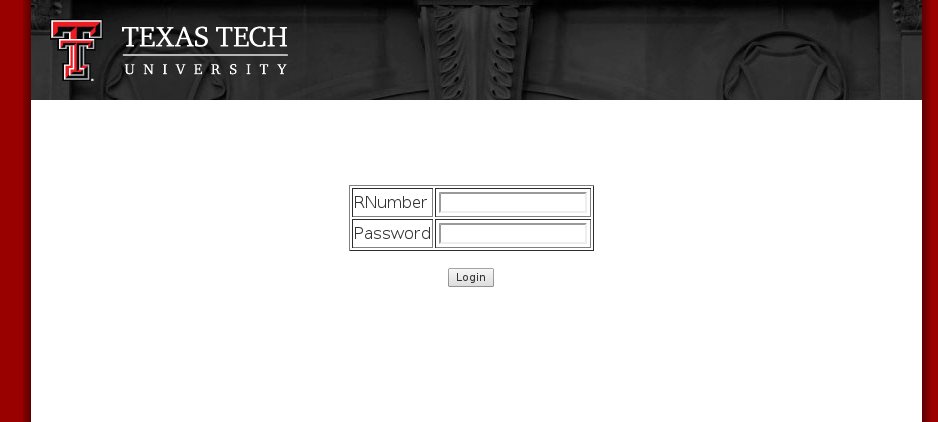
\includegraphics[scale=0.5]{Login.png}
	\caption{Login Page}
\end{figure}

\newpage
\subsection{Edit Template}
The Edit template contains the standard background template and edit table.
\begin{figure}[H]
  	\centering
  	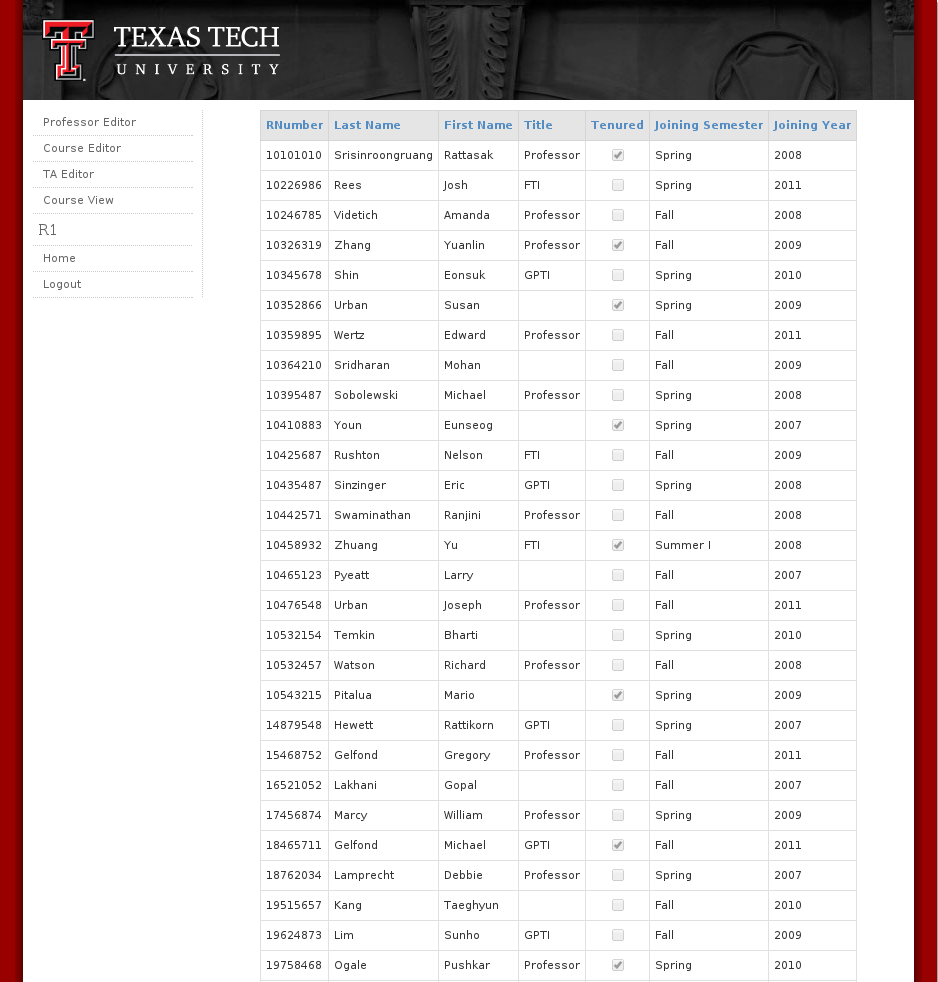
\includegraphics[scale=0.5]{ProfessorEditor.png}
    \caption{Professor Edit Page}
\end{figure}

\newpage
\subsection{View Template}
The view template contains the standard background template and output table.
\begin{figure}[H]
	\centering
	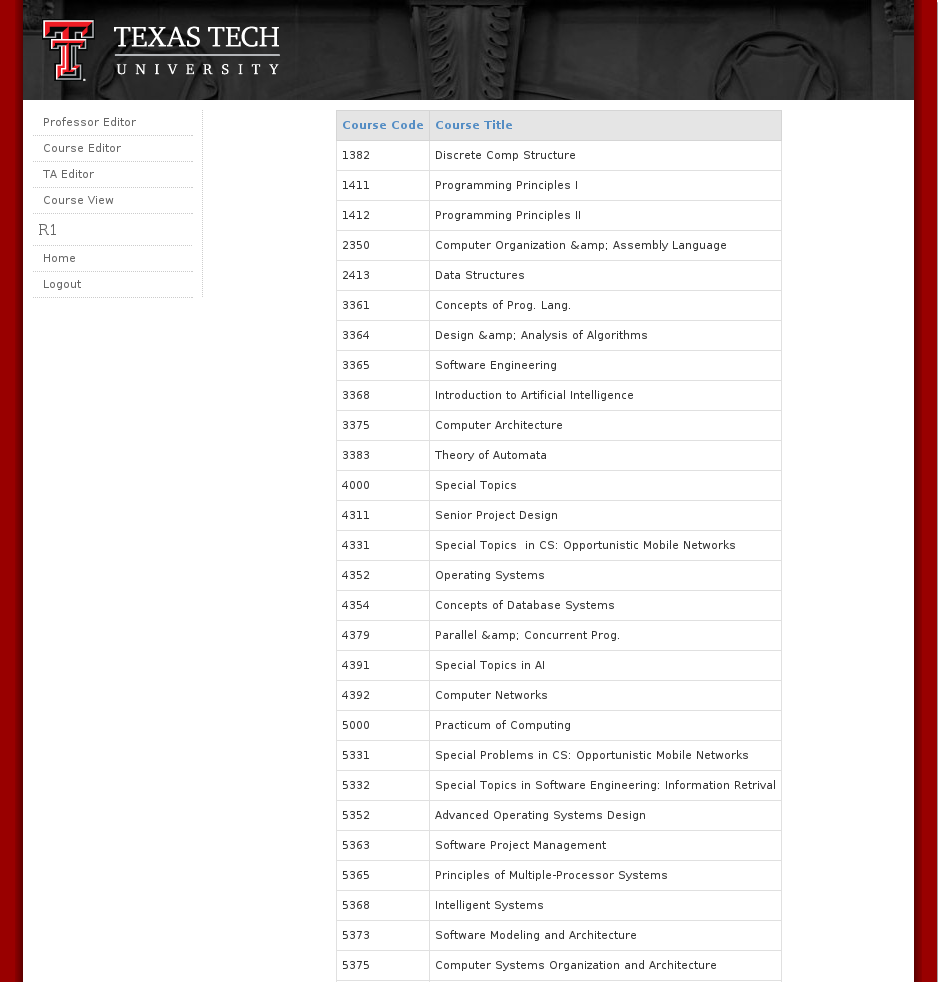
\includegraphics[scale=0.5]{CourseView.png}
	\caption{Course View Page}
\end{figure}
\section{Typography}
The typefaces style has been written to automatically format attractive, readable headers and paragraphs with the following substitutions:\\

\noindent\textbf{High-level headers and some major introductory paragraphs}\\
Arial\\

\noindent\textbf{General content and lower-level headers}\\
Arial

\section{Color}
The page template colors are Texas Tech Dark Red and Texas Tech Black official colors. This is the primary palette used to represent Texas Tech University.	
\begin{figure}[h!]
  	\centering
  	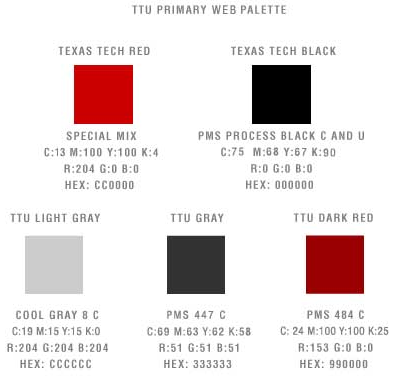
\includegraphics[scale=1]{Capture.PNG}
	\caption{Texas Tech Color Pallet}
\end{figure}